%!TEX root = ../tesi.tex

\chapter{Test e Risultati}
\label{ch:testerisultati}

In questo capitolo vengono presentati e commentati i test effettuati sui moduli di libreria del progetto. 
Per prima cosa viene presentata la struttura dell'impianto di test, sia da lato client che da lato server, successivamente vengono presentati i risultati ottenuti e le problematiche emerse durante lo sviluppo.


\section{Struttura dei test}
\label{sec:strutturatest}
La fase di testing del progetto \`e stata indirizzata alla verifica del corretto funzionamento dei meccanismi implementati all'interno dei moduli esplicati nel capitolo precedente, in particolare il sistema dei dataset sostitutivi e dell'update dei dati ricevuti tramite la connessione di rete, e che attraverso essi fosse possibile produrre un corretto output visivo. Oltre a ci\`o sono stati elaborati con l'obbiettivo di riprodurre i test presenti all'interno del progetto \textbf{SF20LiteTestWorld}, che consiste in un modulo di estensione del framework volto a semplificare la gestione delle finestre grafiche da parte delle applicazioni. Questo modulo \`e ancora in via di sviluppo e per questo non \`e ancora parte integrante delle funzionalit\`a base offerte dallo \ac{SF}, ma il codice relativo ad esso \`e disponibile alla stessa fonte della versione del framework indicata al paragrafo \ref{sub:sfsource}.
I test presenti in questo modulo sono stati pensati non solo per verificare la correttezza delle funzionalit\`a, ma anche per mostrare alcune delle capacit\`a del framework stesso.

Per evitare una eccessiva duplicazione del codice le classi di implementazione dei test, sia lato client che lato server, sfruttano l'ereditariet\`a da una classe genitore comune per condividere tutte le funzionalit\`a comuni.

In figura \ref{f:abstractclient} possiamo vedere la gerarchia delle classi dei client di test, da notare che per implementare un qualsiasi test \`e sufficiente creare una sottoclasse di \texttt{AbstractClient} e implementare al suo interno i metodi astratti della classe genitore. 
\begin{figure}
\begin{center}
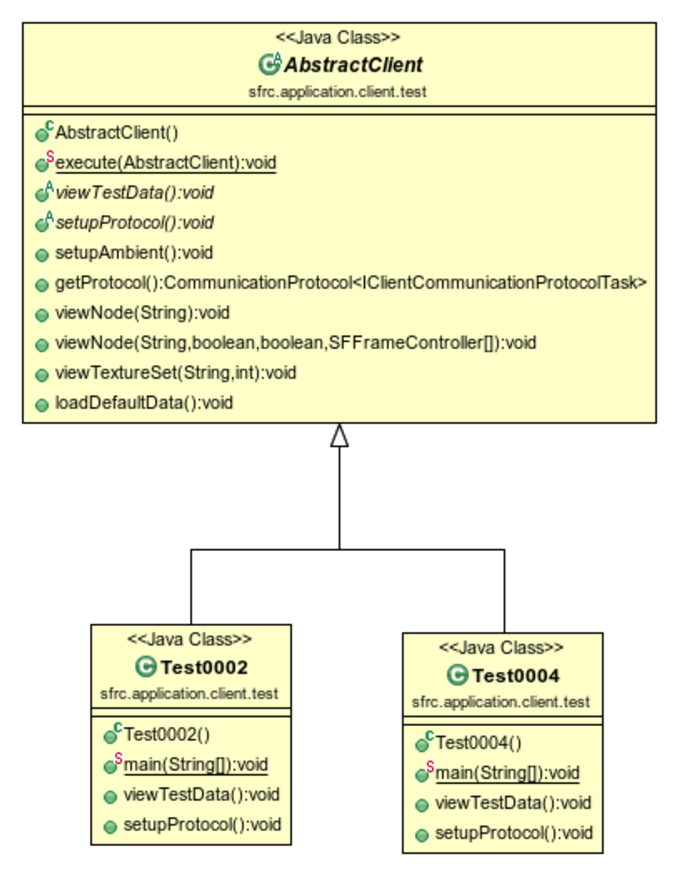
\includegraphics[scale=0.85]{Immagini/abstractclient}
\caption{Gerarchia delle classi di implementazione dei client.\label{f:abstractclient}} 
\end{center} 
\end{figure}
In maniera del tutto simile \`e possibile vedere in figura \ref{f:abstractserver} lo stesso principio applicato per l'implementazione di differenti server di test che opportunamente configurati possono essere usati per riprodurre diverse condizioni a cui il client pu\`o essere sottoposto durante la comunicazione, ad esempio generando dei ritardi di risposta o l'assenza di alcuni dati.
\begin{figure}[t]
\begin{center}
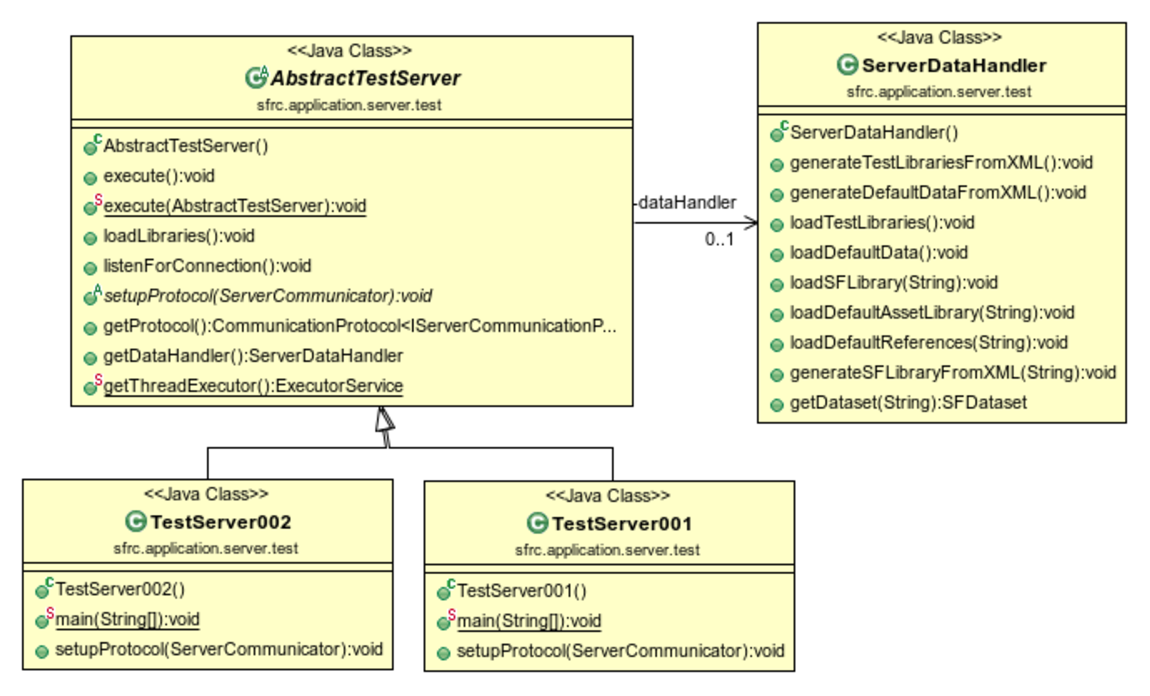
\includegraphics[scale=0.75]{Immagini/abstractserver}
\caption{Gerarchia delle classi di implementazione dei server.\label{f:abstractserver}} 
\end{center} 
\end{figure}
In quest'ultima figura \`e evidenziata la classe \texttt{ServerDataHandler}, la quale si occupa di effettuare la gestione dei dati sul server in esecuzione dato che, non essendoci la necessit\`a di renderizzare i dati tridimensionali, non \`e necessario utilizzare un'infrastruttura centralizzata complessa come quella del DataCenter del framework.

Le classi che implementano i test sono contenute nei package \\\texttt{sfrc.application.client.test} e \texttt{sfrc.application.server.test}.

\section{Test significativi}
\label{sec:test}
Il server di test utilizzato nelle prove descritte di seguito \`e il \textbf{TestServer002} ed \`e stato configurato per avere tre secondi di ritardo tra la risposta di una richiesta ed un'altra. Questa configurazione permette di osservare nel dettaglio la reazione dei meccanismi implementati ad un arrivo progressivo dei dati.

\subsection{Test0006}
Questo test ha l'obbiettivo di visualizzare all'interno di una finestra, tre oggetti che condividono una geometria dalla forma di fungo e su cui sono applicate delle texture. Sia la geometria che le texture sono generate proceduralmente durante l'esecuzione usando la capacit\`a di calcolo della \ac{GPU}.
\begin{figure}%[t]
\begin{center}
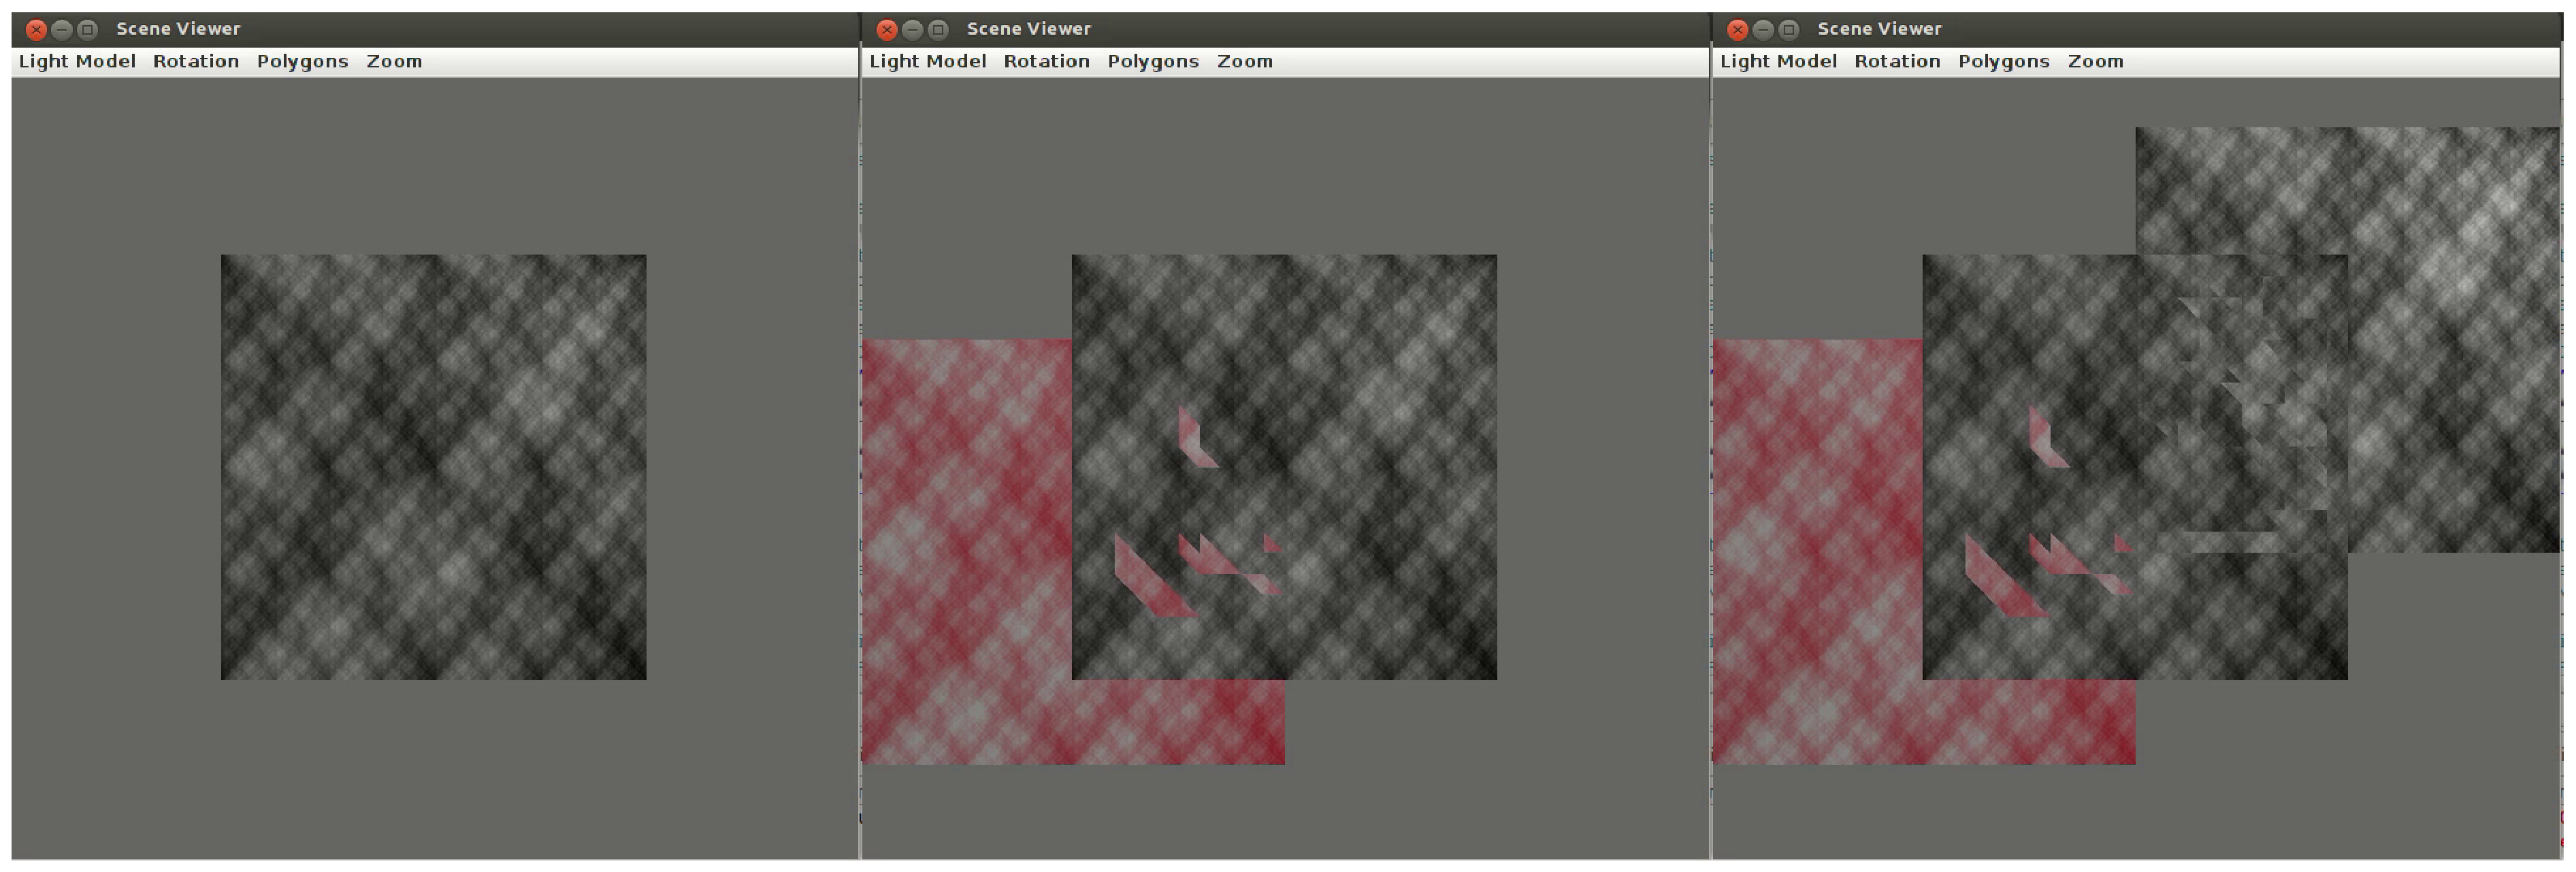
\includegraphics[width=\textwidth]{Immagini/test0006/test0006-wall1}
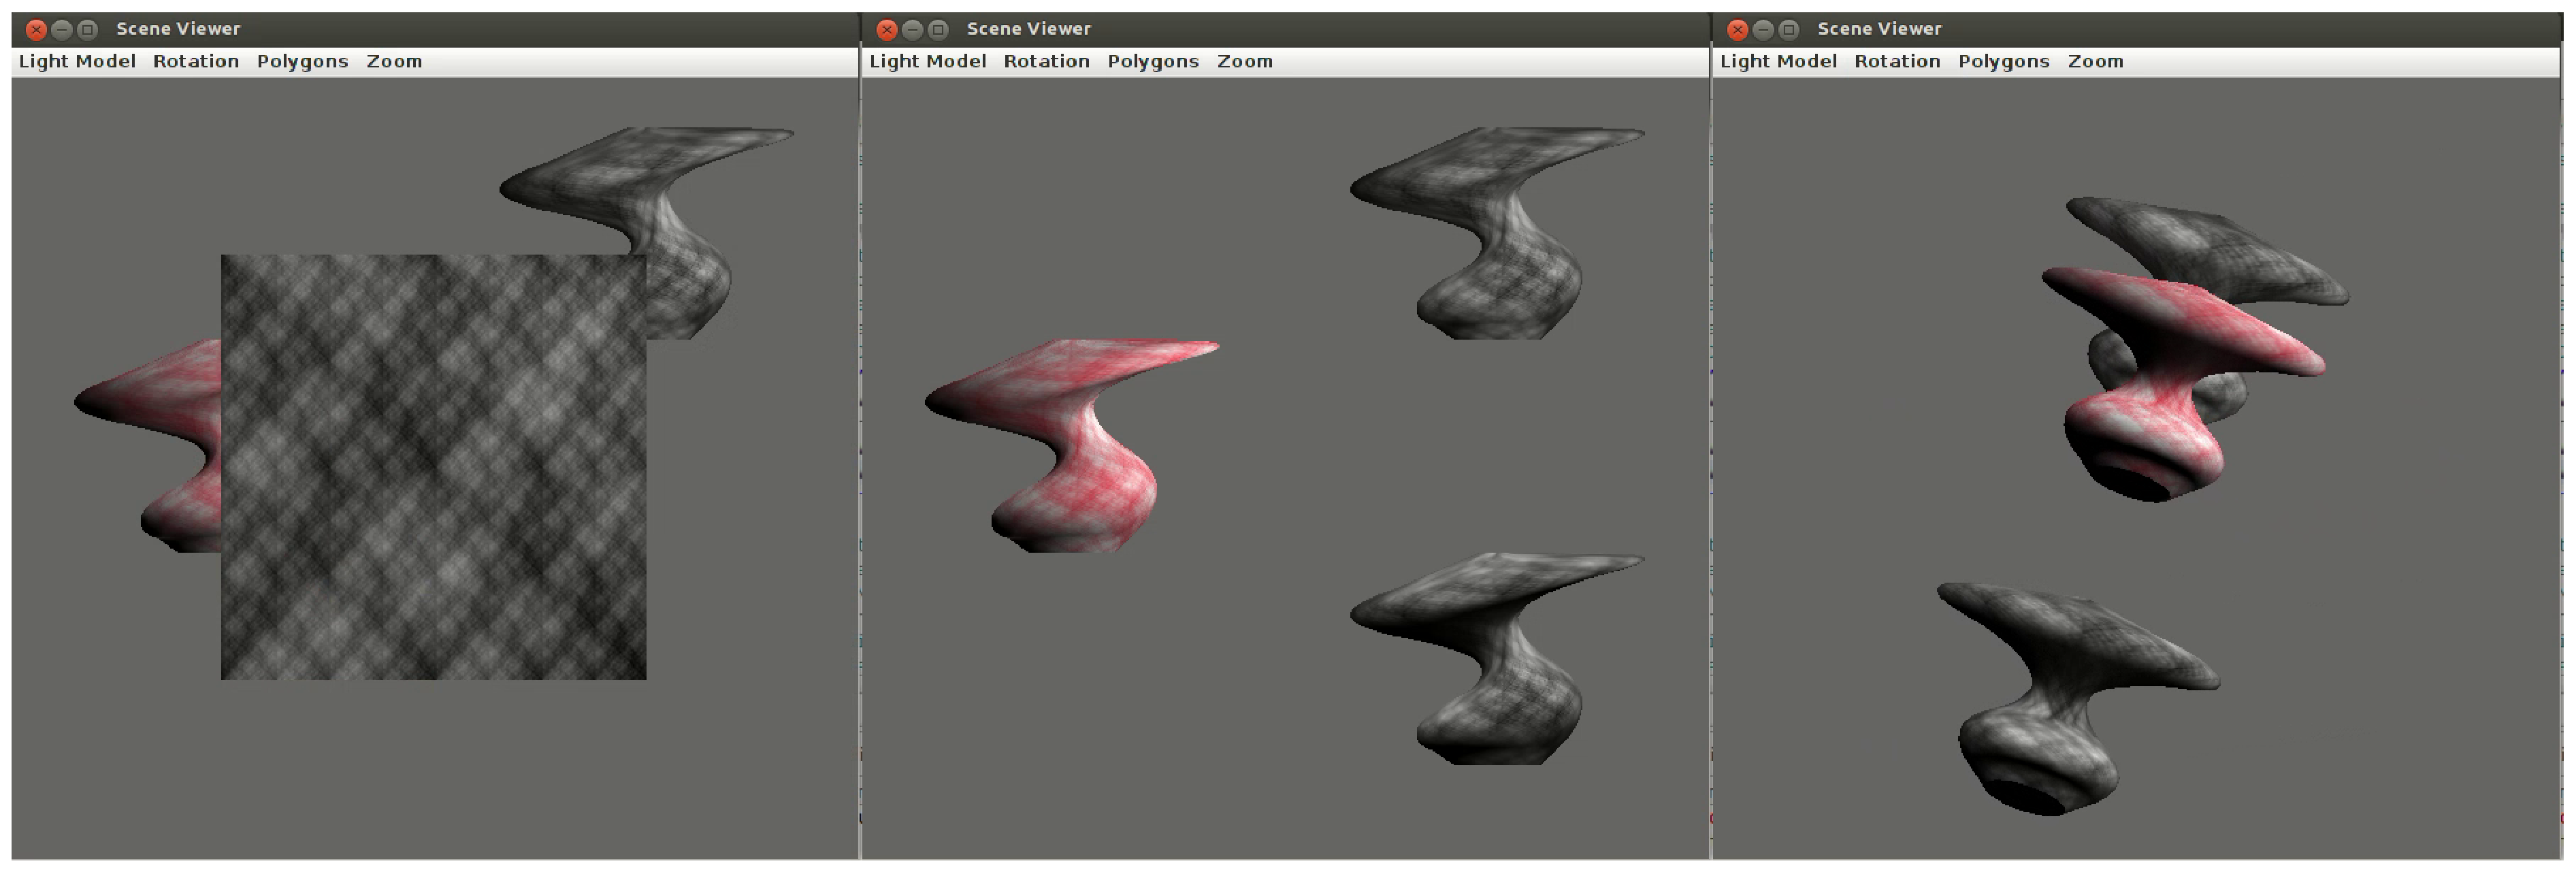
\includegraphics[width=\textwidth]{Immagini/test0006/test0006-wall2}
\caption{Fotogrammi estratti dall'esecuzione del test Test0006. \label{f:test0006-wall}} 
\end{center} 
\end{figure}
In figura \ref{f:test0006-wall} viene mostrata una sequenza di fotogrammi dell'esecuzione del test: al lancio dell'applicazione (fig.\ref{f:test0006-wall} in alto a sinistra) la scena richiesta viene temporaneamente sostituita con un'altra che contiene un semplice cubo texturizzato. 
Al loro arrivo, i dati della scena reale che contengono i riferimenti ai tre oggetti vengono analizzati generando la richiesta degli oggetti verso il server mentre nel frattempo ognuno viene sostituito con un cubo posto al centro della scena. Questa sostituzione non genera un cambiamento visibile in quanto i tre cubi sono sovrapposti e posizionati esattamente come quello contenuto nella scena sostitutiva.

Quando i dati del primo oggetto vengono ricevuti (fig.\ref{f:test0006-wall} in alto al centro) vengono immediatamente applicati alla scena: possiamo notare il cambiamento di colore e la traslazione di un cubo verso sinistra. 
L'oggetto non cambia forma perch\`e il pacchetto di informazioni contiene un riferimento alla geometria ``fungo'' generica ancora non presente e per cui viene generata una richiesta. 
Nel fotogramma successivo (fig.\ref{f:test0006-wall} in alto a destra) vediamo gli effetti dell'arrivo del pacchetto di informazioni relativo al secondo oggetto: un'altro cubo viene traslato, stavolta verso destra. 
L'informazione sulla geometria ``fungo'' non \`e ancora arrivata, ma non viene generata una nuova richiesta dato che il sistema ha gi\`a una richiesta pendente, l'oggetto viene invece registrato per un update della geometria.
Nel quarto fotogramma (fig.\ref{f:test0006-wall} in basso a sinistra) finalmente arriva la geometria e tutti gli oggetti che si erano registrati per un update vengono aggiornati, da notare che non avendo ancora ricevuto i dati relativi al terzo oggetto esso rimane nella sua forma sostitutiva. Questo accade grazie al parallelismo dei processi che effettuano le richieste, che consente di non dover necessariamente ricevere i dati in un ordine specifico.
Nella penultima immagine (fig.\ref{f:test0006-wall} in basso al centro) si vede l'aggiornamento visivo all'arrivo delle informazioni sul terzo oggetto, avendo gi\`a ricevuto i dati della geometria essa viene applicata immediatamente insieme alla traslazione. Nell'ultimo fotogramma vediamo la scena finale ruotata dai controlli della finestra client, per effettuare la navigazione della scena non \`e pi\`u necessario richiedere altri dati al server e le connessioni vengono chiuse.

Per non appesantire la precedente descrizione si \`e omesso che durante l'esecuzione sono stati richiesti e trasferiti anche i dati relativi alle texture da applicare ai modelli, la transizione non \`e direttamente visibile dato che le texture sostitutive hanno la stessa trama e non sono visivamente distinguibili.

\subsection{Test0019}
Questo test prevede la visualizzazione di un oggetto avente geometria a fungo a cui viene applicata una texture e una bumpmap\footnote{Una bumpmap \`e un particolare tipo di texture che viene utilizzata tramite la tecnica del BumpMapping. Questa tecnica si serve delle informazioni della bumpmap per descrivere la variazione da applicare al vettore normale di ogni punto di una superficie a cui \`e applicata. Ci\`o permette di ottenere l'effetto visivo di superfici irregolari senza per\`o effettivamente spostare i vertici della superficie stessa}. Anche in questo caso sia la geometria che le texture sono ottenute proceduralmente attraverso il rendering della \ac{GPU}.

\begin{figure}%[t]
\begin{center}
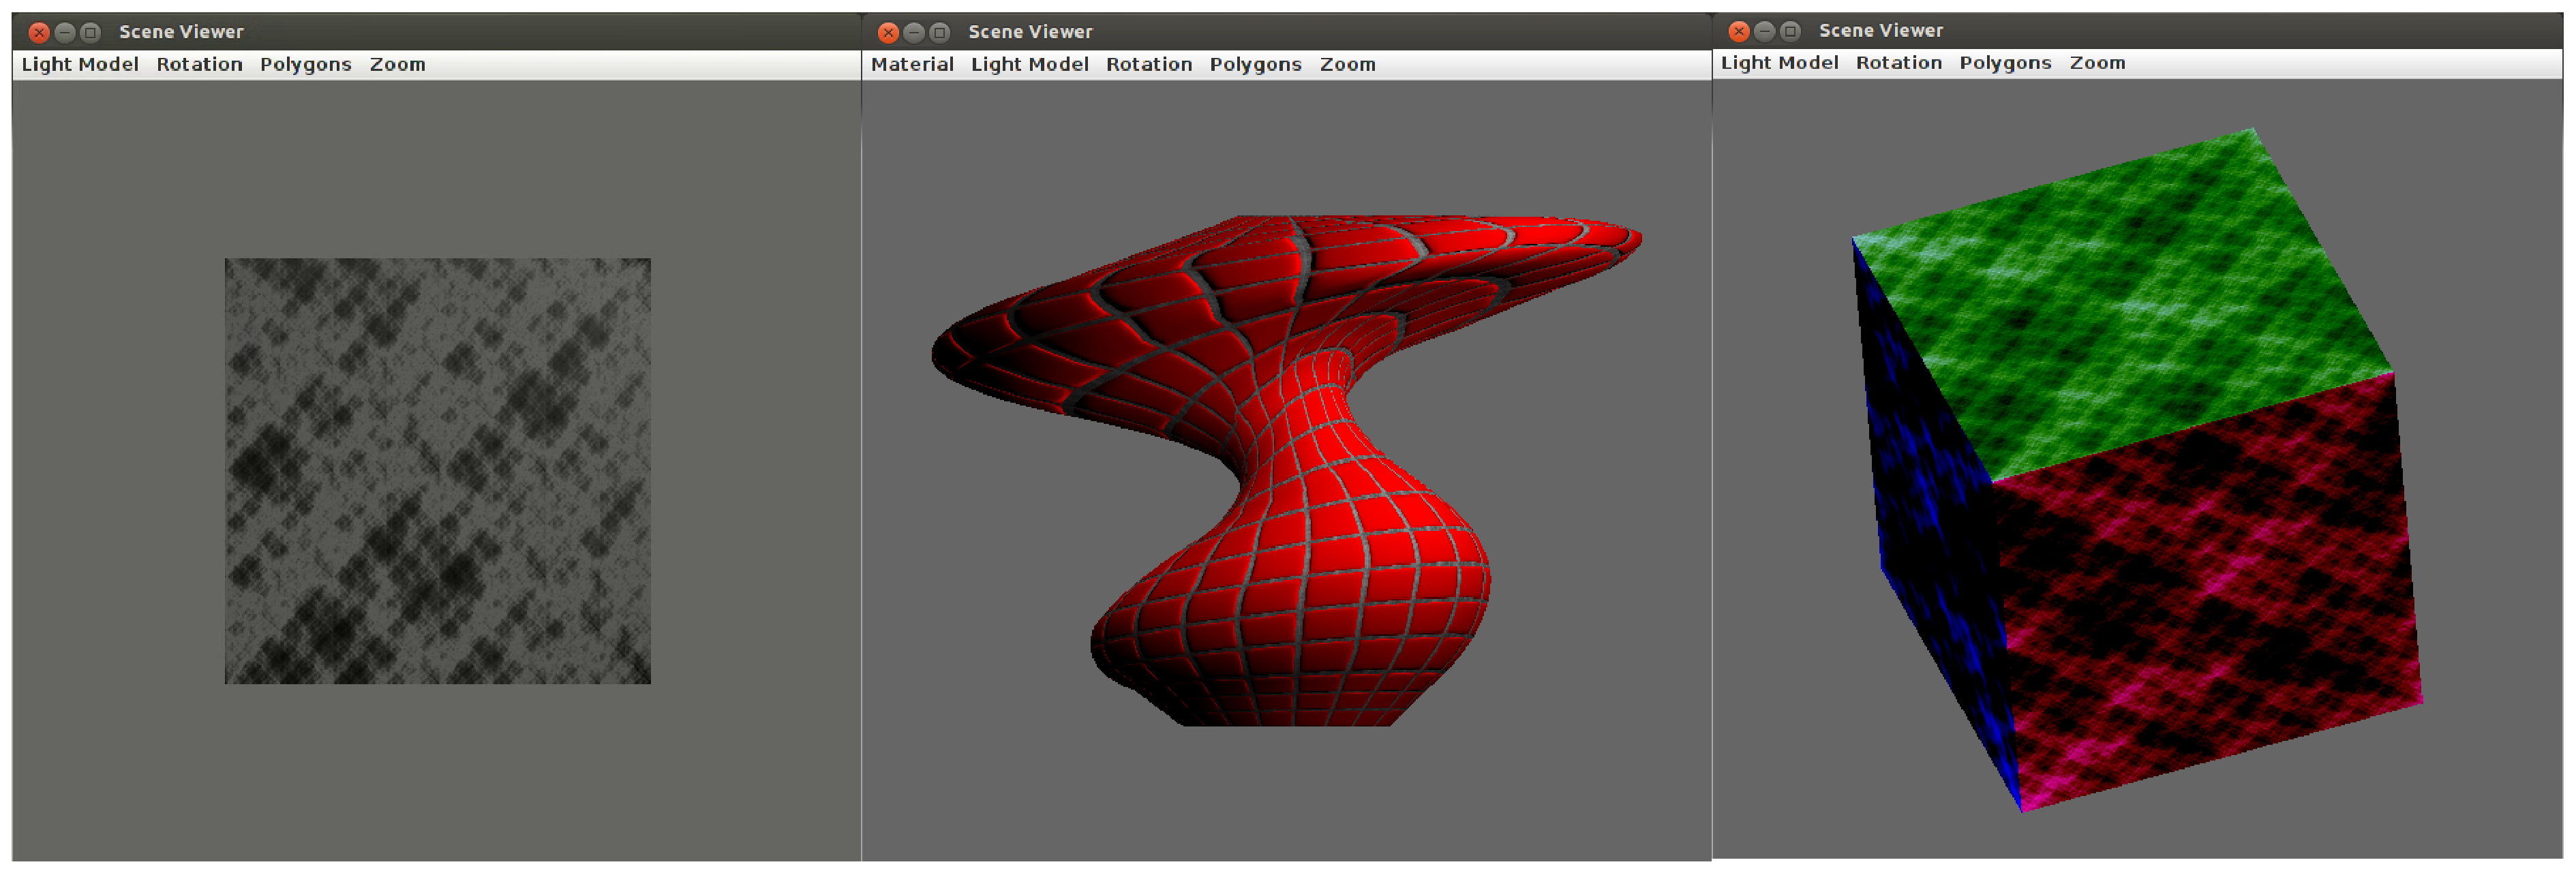
\includegraphics[width=\textwidth]{Immagini/test0019/test0019-wall1}
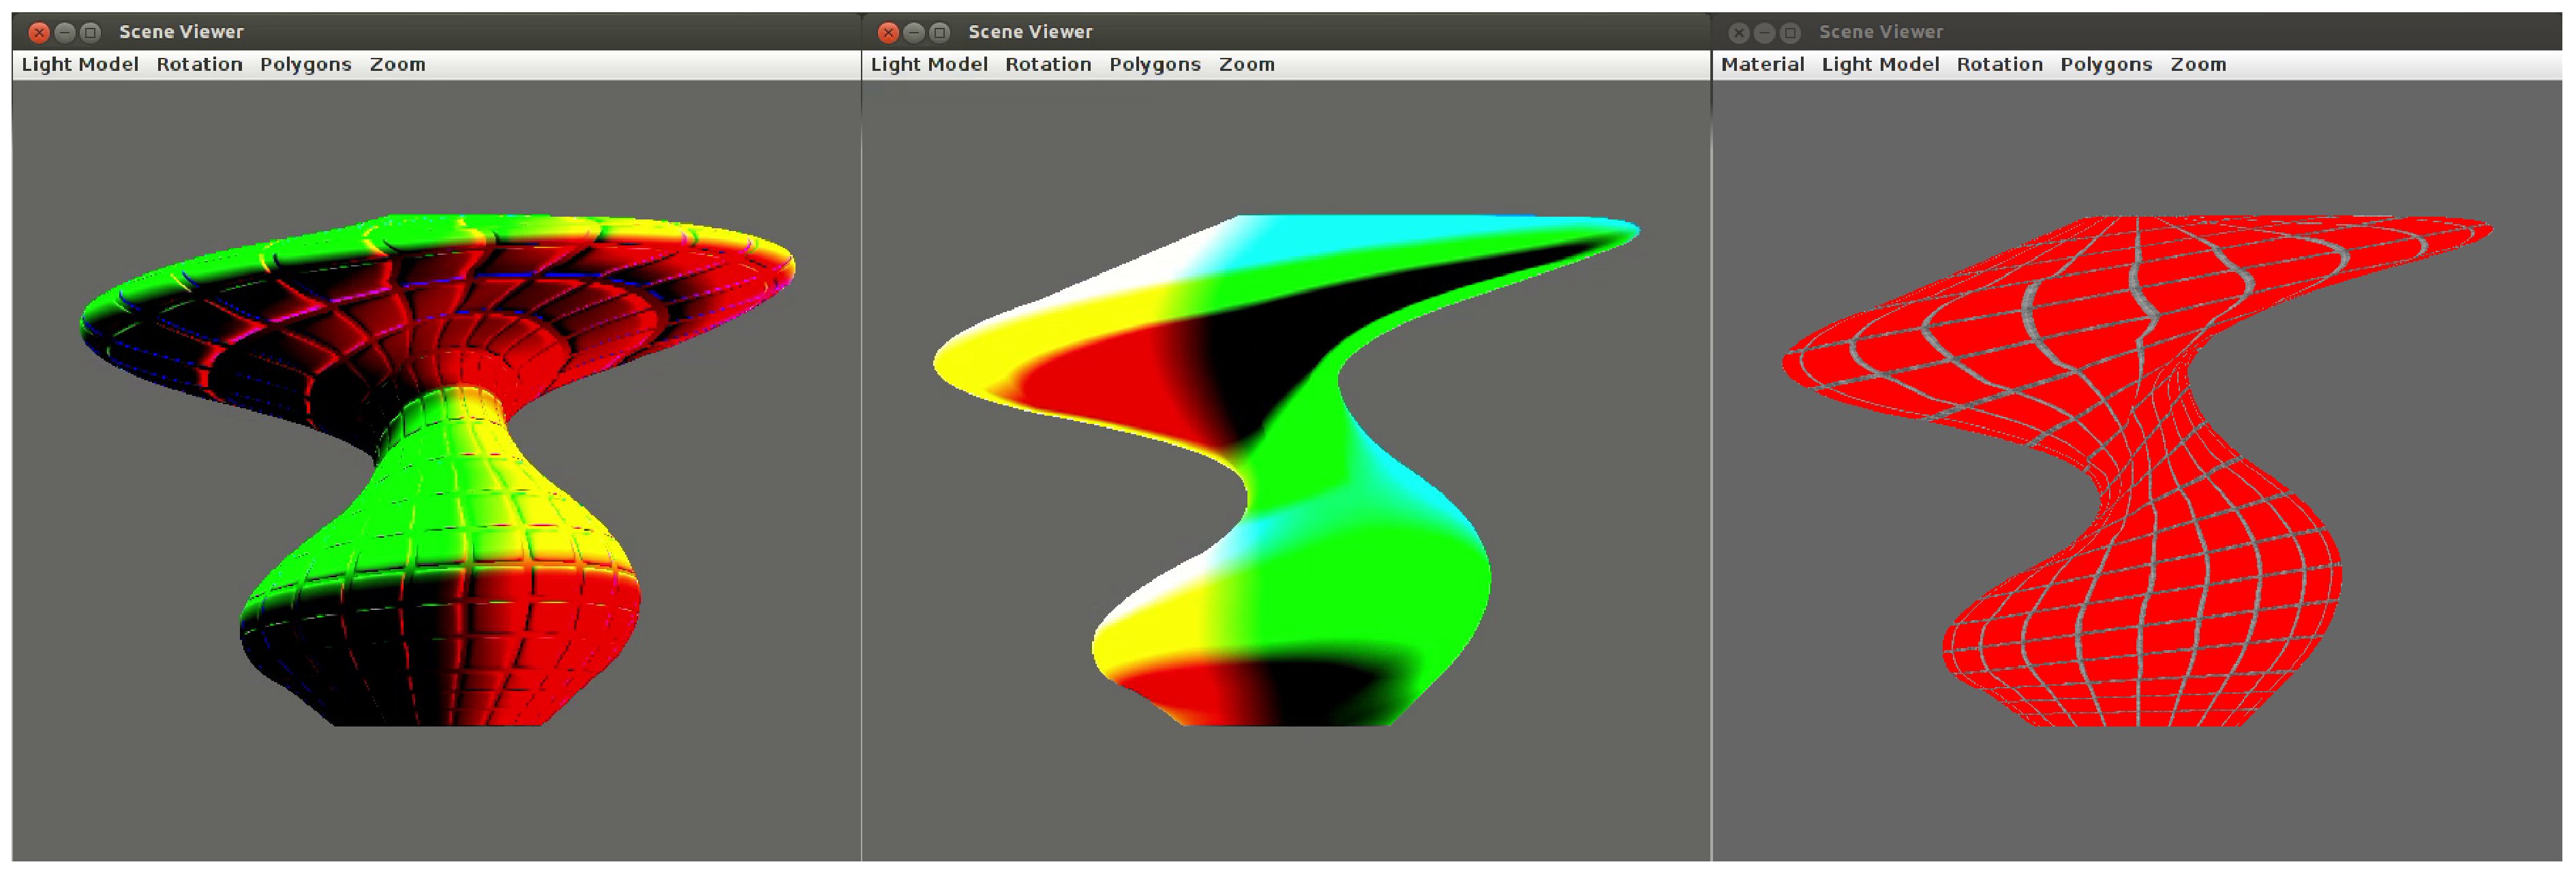
\includegraphics[width=\textwidth]{Immagini/test0019/test0019-wall2}
\caption{Fotogrammi estratti dall'esecuzione del test Test0019. \label{f:test0019-wall}} 
\end{center} 
\end{figure}



\begin{figure}%[t]
\begin{center}
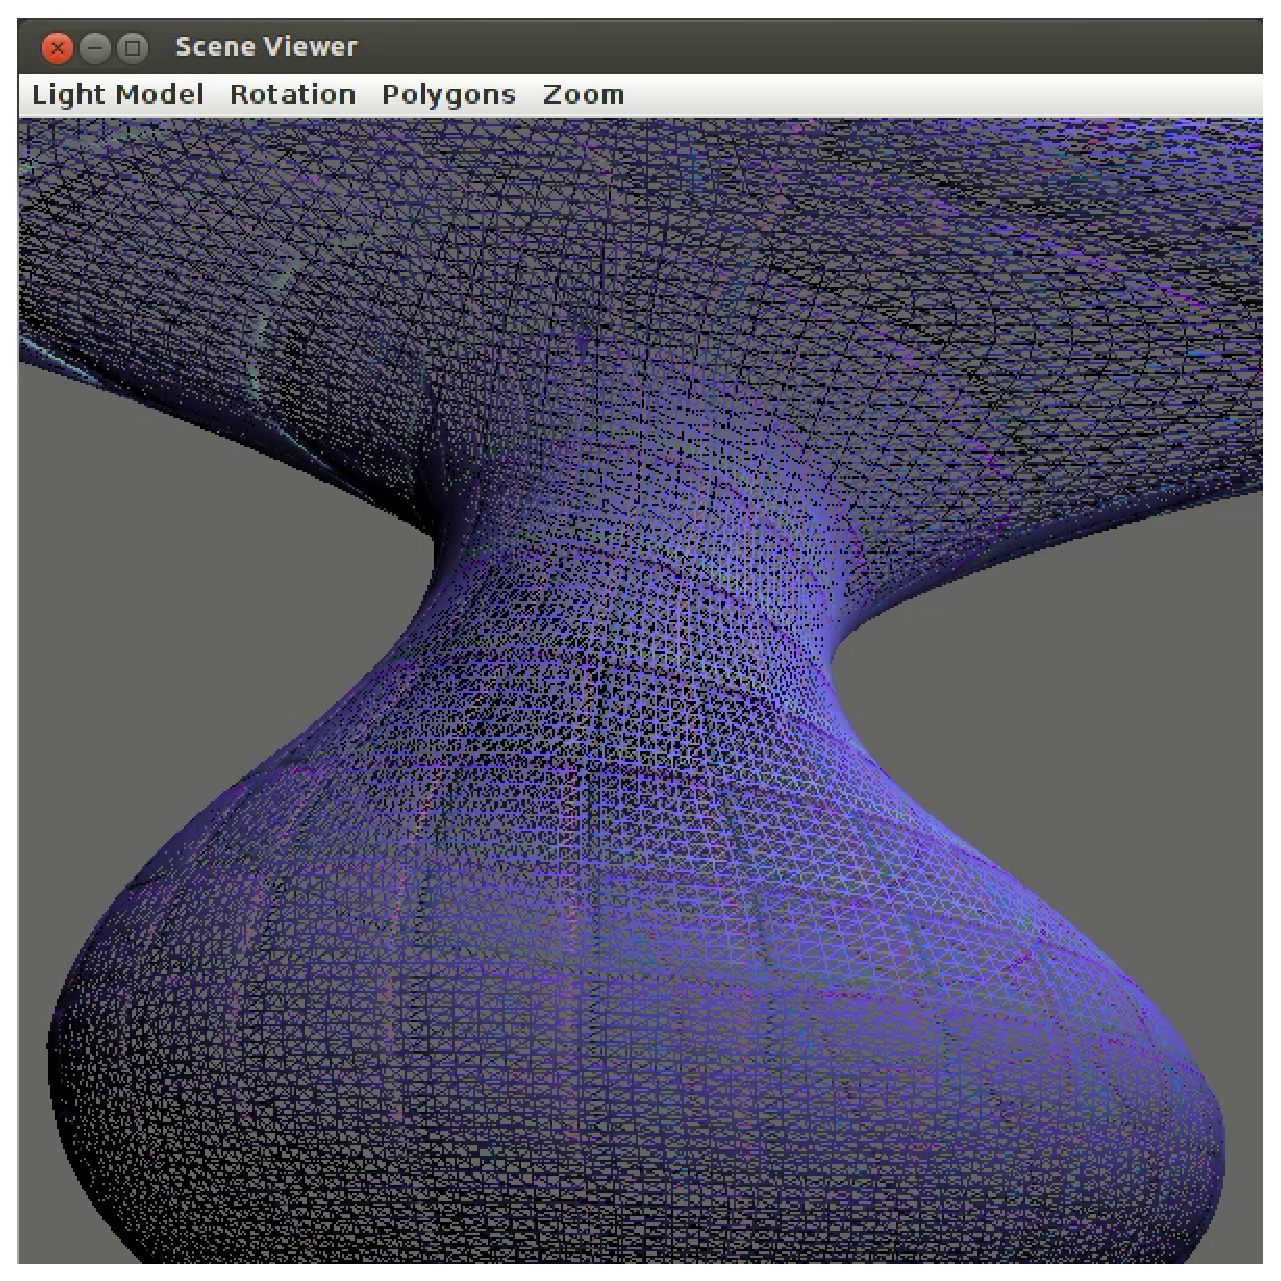
\includegraphics[width=\textwidth]{Immagini/test0019/test0019-tessel}
\caption{Particolare di un fotogramma estratto dall'esecuzione del test Test0019, \`e posta in evidenza la tassellazione in triangoli operata sul modello del fungo. \label{f:test0019-tessel}} 
\end{center} 
\end{figure}

\section{Attivit\`a correlate}
\label{sec:correlate}
La variet\`a dei contenuti dei test di riferimento ha reso necessario un lavoro aggiuntivo orientato alla creazione di un insieme di dataset sostitutivi da inserire nella libreria di oggetti di default usati come rimpiazzo temporaneo.

